\documentclass{tufte-handout}

\title{On ultimate: dumps and retaining possession}
\author[James Reynolds]{James Reynolds}

%\date{28 March 2010} % without \date command, current date is supplied

%\geometry{showframe} % display margins for debugging page layout

\usepackage{graphicx} % allow embedded images
  \setkeys{Gin}{width=\linewidth,totalheight=\textheight,keepaspectratio}
  \graphicspath{{graphics/}} % set of paths to search for images
\usepackage{amsmath}  % extended mathematics
\usepackage{booktabs} % book-quality tables
\usepackage{units}    % non-stacked fractions and better unit spacing
\usepackage{multicol} % multiple column layout facilities
\usepackage{lipsum}   % filler text
\usepackage{fancyvrb} % extended verbatim environments
  \fvset{fontsize=\normalsize}% default font size for fancy-verbatim environments

% Standardize command font styles and environments
\newcommand{\doccmd}[1]{\texttt{\textbackslash#1}}% command name -- adds backslash automatically
\newcommand{\docopt}[1]{\ensuremath{\langle}\textrm{\textit{#1}}\ensuremath{\rangle}}% optional command argument
\newcommand{\docarg}[1]{\textrm{\textit{#1}}}% (required) command argument
\newcommand{\docenv}[1]{\textsf{#1}}% environment name
\newcommand{\docpkg}[1]{\texttt{#1}}% package name
\newcommand{\doccls}[1]{\texttt{#1}}% document class name
\newcommand{\docclsopt}[1]{\texttt{#1}}% document class option name
\newenvironment{docspec}{\begin{quote}\noindent}{\end{quote}}% command specification environment

\begin{document}

\maketitle% this prints the handout title, author, and date

%\printclassoptions

\newthought{Defence wins games; 
offence loses them.}
In ultimate 
the scoring team 
pulls 
to start the next point, 
except 
(sometimes) 
after half.
Hence, 
the difference
in the number 
times possession
is lost 
(i.e. a turnover)
by each team
is related to 
the difference in 
the scores\footnote{
Let A 
be the score of 
the team with the
highest score,
and  B be the 
score of the 
other team; 
and let 
C and D
be the number
times possession
is lost 
by the team
with the highest score
and the other team, 
again respectively. 
Then, 
during the first half, 
at the end 
of a point when 
A + B is odd
or even, 
respectively, 
Equations 1 
or 2 
apply. 
After half,
mirroring 
makes it all
too confusing 
to both with 
formal equations, 
as the same principles
apply.}. 


\begin{marginfigure}
\begin{equation}
A - C = 1 - B - D
\end{equation}
\end{marginfigure}
\begin{marginfigure}
\begin{equation}
A - C = B - D
\end{equation}
\end{marginfigure}



A team 
that (somehow)
never loses 
possession across
an entire game 
will defeat 
a team 
that loses possession 
only once or twice\footnote{
Again, 
there are edge cases 
related to 
winning the toss and
mirror at half, 
and very windy days.}, 
Hence, 
being able 
to retain possession 
is important\footnote{
More important than getting 
a big layout block on 
defence? Possibly, 
because at that point 
the job 
is only half done - 
your team still 
needs to convert 
the block into a goal!},
especially on 
points when 
your team 
receives 
the pull. 

\newthought{What is a dump and why is it important?}
A backwards pass?  
A short pass?  
A pass 
to a handler?
It might be 
one 
or all 
of these, 
Typically 
a dump 
is used to 
reset the stall count,
retain possession, 
and/or improve 
the position
of the disc.  
Being able 
to complete 
dump throws 
is important because 
this impacts, 
and to an extent dictates, 
whether your team can 
play low-risk, high-completion 
offense. 
With an effective dump-set 
your team can retain possession
and wait for  
good opportunities.  
Without a reliable dump-set, 
you'll likely 
need to play higher-risk 
offence\footnote{
Huck-and-zone anyone? 
Not that there is anything 
wrong with huck-and-zone 
if it is working. 
Just that it 
will
probably
not work 
against teams
who don't turn the disc over much. 
Having an 
effective 
dump-set 
means your team 
probably 
gets to choose 
whether to 
play a
high- or 
low-risk 
style 
of offence. 
If you can't 
reliably 
make dumps, 
then your
strategic options 
are more limited.}.  

The probability 
of losing possession
is a function of 
the number of passes made 
and the completion rate of 
each of those passes\footnote{
For example,  
if it takes 5 throws
to score and 
each has a 85\% chance 
of being completed
the overall chance 
of scoring is only 44\%.
Compared to this, 
a 50-50 huck
to the endzone
straight off the pull 
isn't looking too bad.}.
Reality is more complex, 
with
completoin rates 
varying by 
thrower, 
throw 
and situation. 
Plus potential 
\smallcaps{second-order factors},  
where someone 
takes riskier options 
because the average 
completion rate 
for the whole team
is low enough 
that a turnover is 
likely soon anyway.
But, in general, 
if the average completion rate 
goes up, 
everyone will get 
to take less risky options\footnote{
Again,  
if the completion rate 
goes up 
to 95\%, 
we are a 77\% chance 
of scoring if it takes 
5 passes
... and suddenly 
that 50-50 huck 
isn't looking too good anymore. Another way of looking at this 
is: (1) ultimate
is usually stacked towards 
the offence 
(unless 
it is 
excessively 
windy)
because (1a) it is non-contact 
and (1b) there is 
typically 
somewhere
to throw the disc to 
such that a defender 
can't get to it without running 
through the receive; 
and (2) all defences 
will eventually 
break down 
as it is impossible to 
cover everything 
for ever. 
Hence, 
(3) if your team 
can just hold onto
possession 
long enough
low-risk
opportunities to 
advance and/or score
will come.}.

However, 
even though 
the team on offence 
typically
has the advantage 
in ultimate 
(as they choose 
where the disc 
goes next), 
the agenda is 
typically set 
by the team 
on defence, 
because they 
get to choose 
what defensive formation 
to use.
Having possession 
of the disc, 
entails 
reacting 
to what 
the defenders 
do and, 
typically, 
taking what they give you. 
So dumping 
might vary if playing.... 

\newthought{...against zone defences},
which typically
involve defenders 
covering space, 
rather than 
specific individuals. 
Dumping is 
especially important 
if you 
are not 
a handler 
so as have
enough 
receivers 
downfield 
to throw to.
Zones come in
many different variations, 
but can typically be 
beaten 
by going \smallcaps{Around}, 
going \smallcaps{over} or 
\smallcaps{through}. 
In Figure \ref{fig:dump_zone}
(left) O6 throws 
\smallcaps{around}
to O5 or O7, 
while in Figure \ref{fig:dump_zone}
(right) O7 throws 
\smallcaps{around} to O6, 
or \smallcaps{through} 
or \smallcaps{over} 
to O5. 
Receivers
might help 
the thrower 
by standing still\footnote{
Thereby allowing 
a no-look, 
or otherwise direct 
and quick,
pass}, 
as they are not 
being marked 
and so there is no one 
to run away from!
Choose your location 
by balancing the 
need to 
limit turnover risk
for the dump throw itself, 
versus 
maximising 
opportunities 
for the next throws\footnote{
For example
in Figure \ref{fig:dump_zone} (right)
the further upfield O6 stands 
the longer the throw 
will need to be 
from O7, but
the more likely 
it will be to make 
the next throw 
(thin line) to O5 
before D12 arrives.}. 



\begin{marginfigure}%
  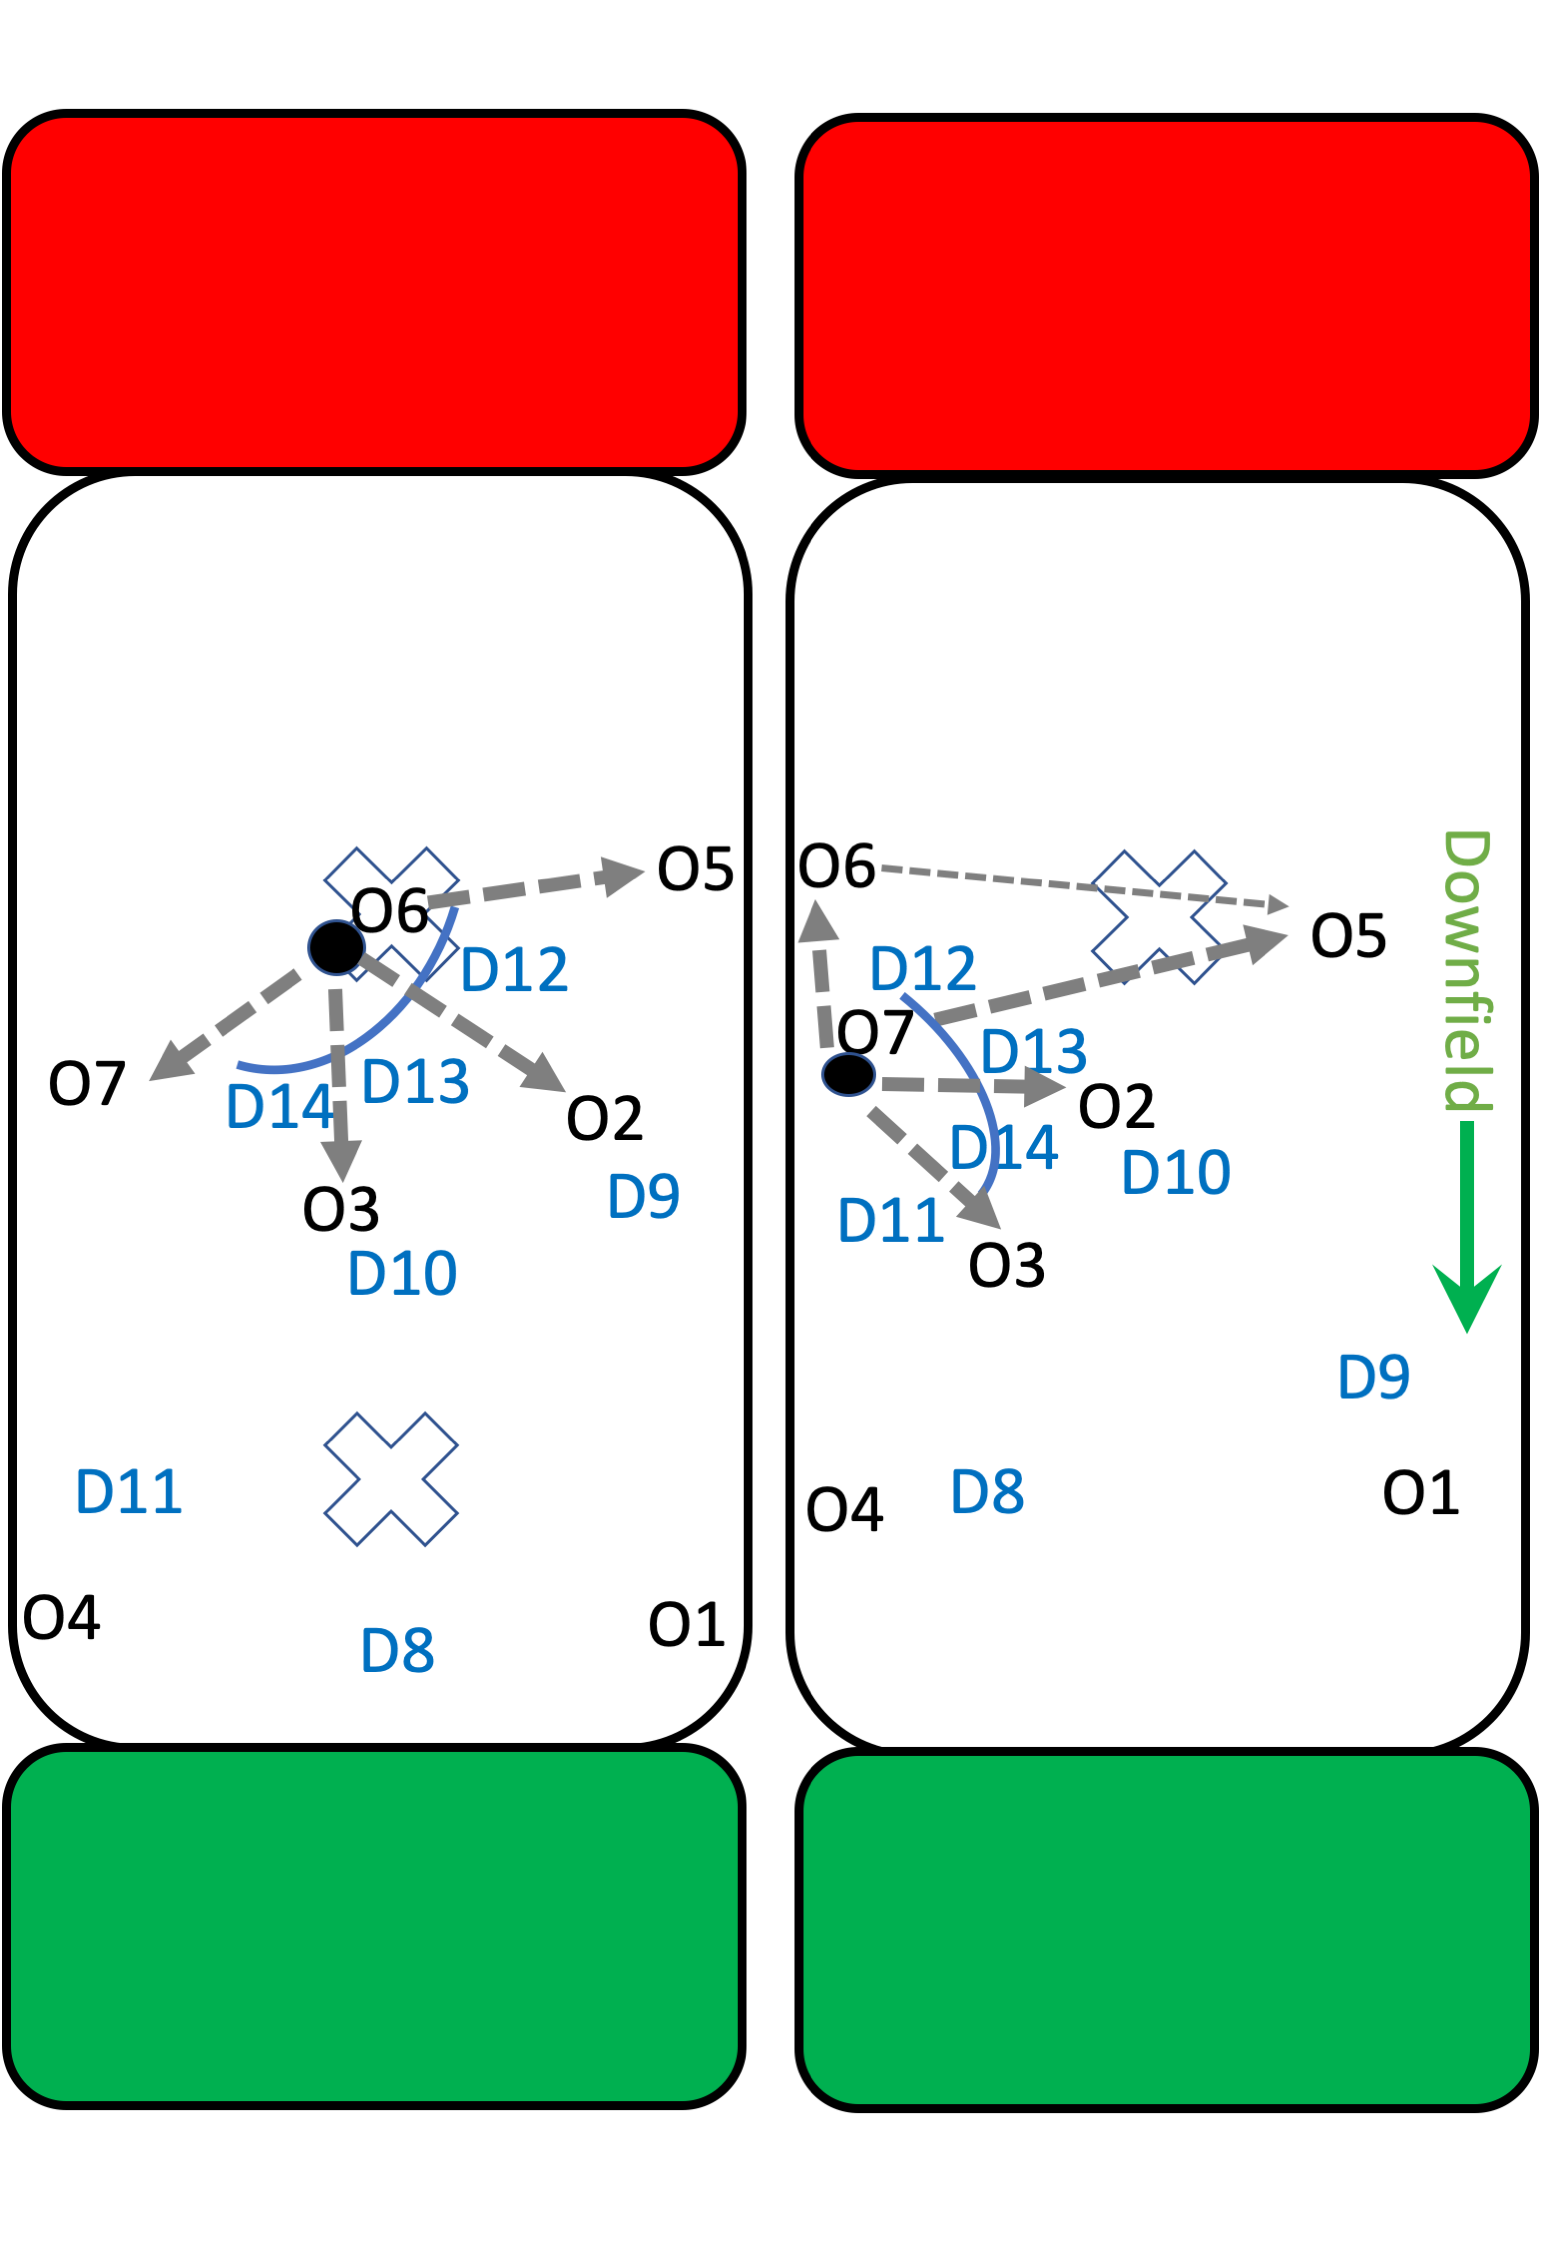
\includegraphics[width=\linewidth]{dump_zone}
 \caption{Dumping vs zones}
 \label{fig:dump_zone}
 \end{marginfigure}



\begin{marginfigure}%
  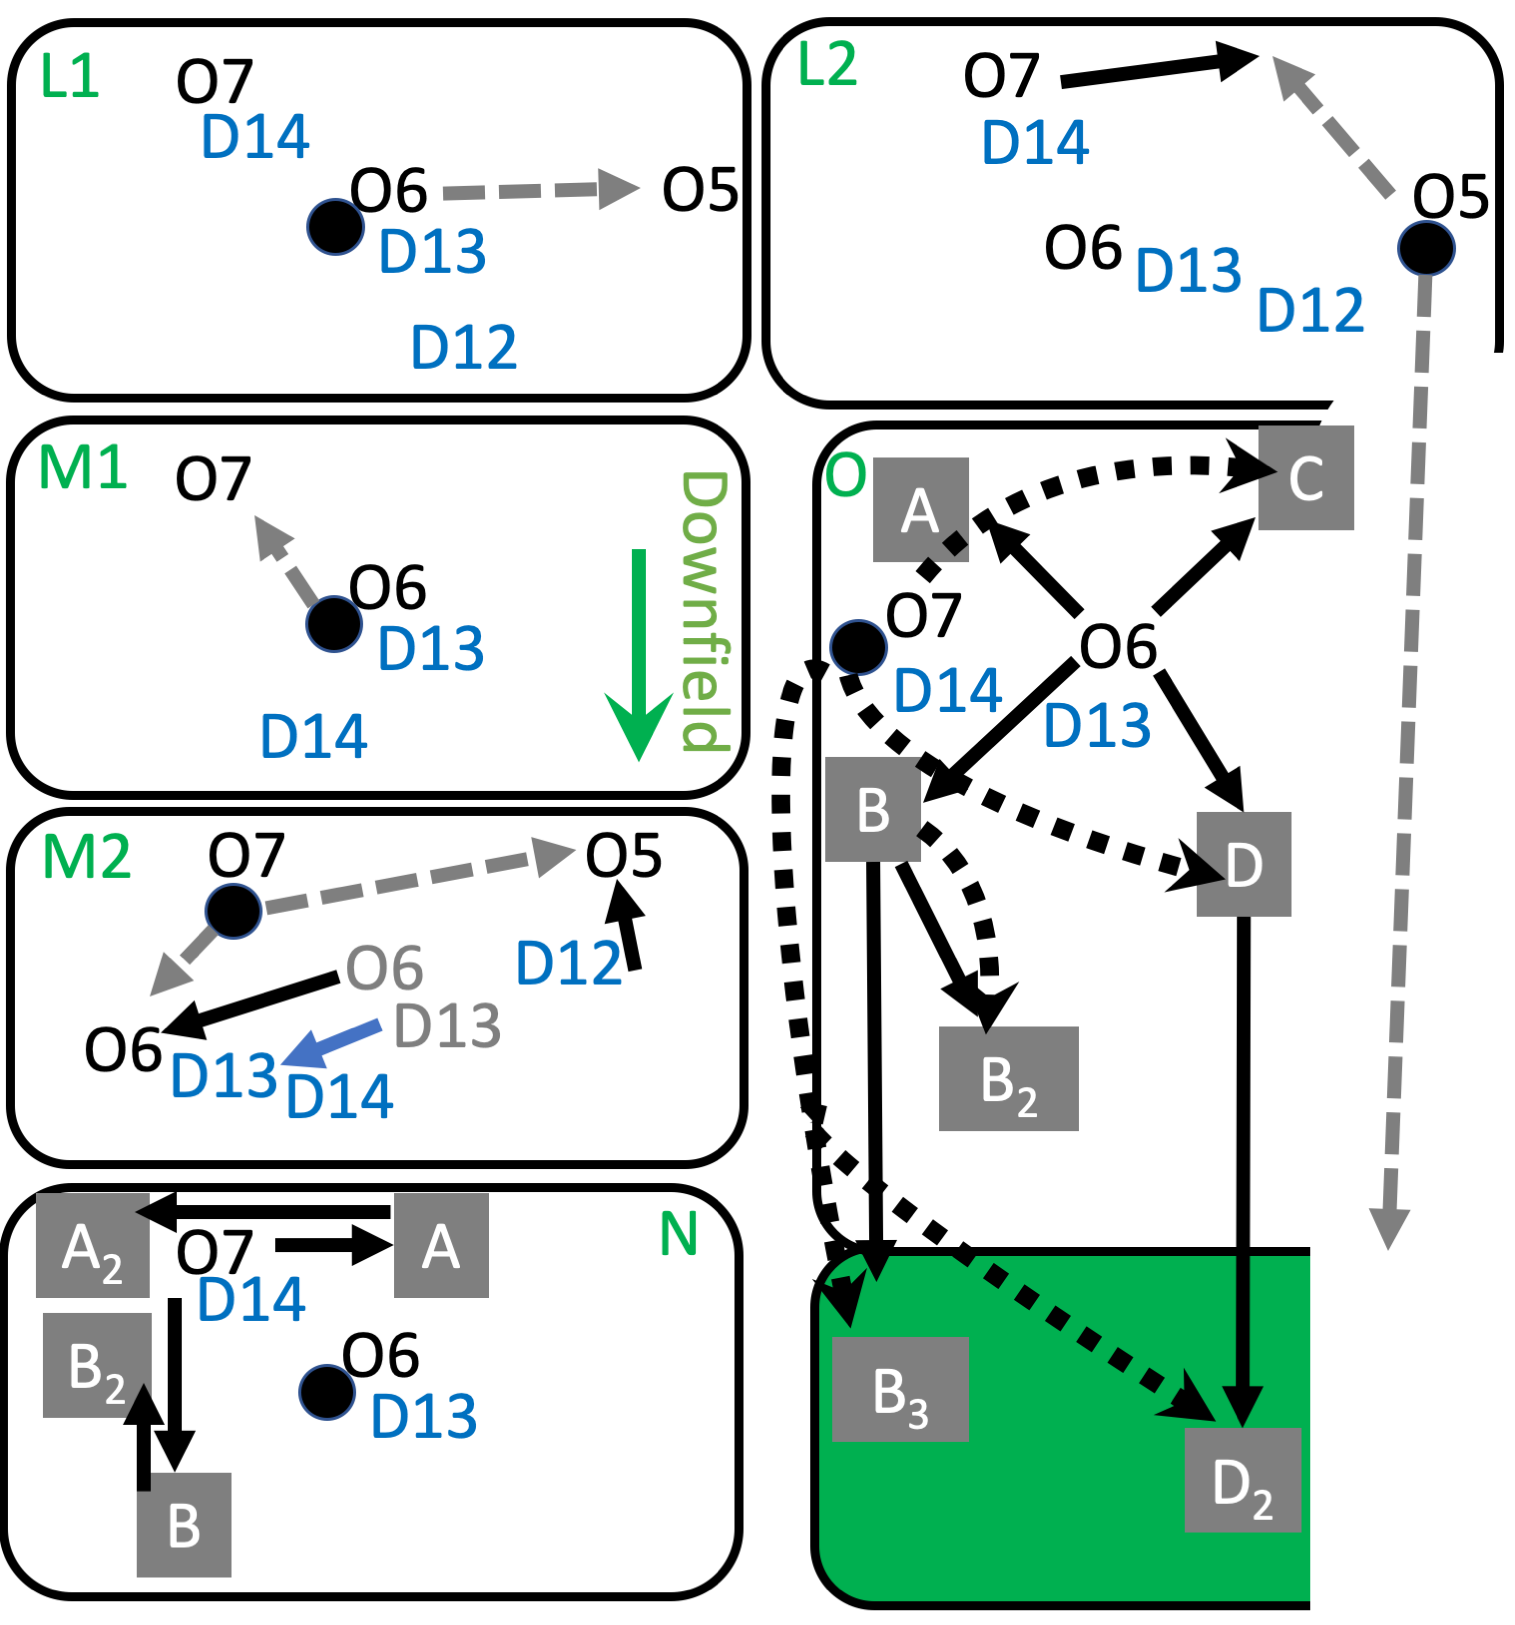
\includegraphics[width=\linewidth]{dump_match}
 \caption{Dumping vs person-match}
 \label{fig:dump_match}
 \end{marginfigure}

\newthought{...Against person-match defences}, which typically involve each defender covering a single offensive player. Figure \ref{fig:dump_match} shows four variations (L, M, N and O).  In L1 D12 has decided to poach off O5, so O5 can move as close to the sideline as possible, receive a pass from O6, and then (in L2) use the time it takes D12 to get across to throw it to virtually anywhere on the field at all! M1 shows the situation where D14 has poached off O7.  However, because O7 set up at a 45 degree angle behind O6 a direct pass (in M1) can be passed back to them or across to O5 (in M2).  D13 is on the wrong side of O6 to be able contest the O7-to-O6 throw and D14 is lost at sea. 

N and O show variations where the defenders are 'being honest' and actually covering their player.  In N O7, again set up at the 45, has opportunities to cut to A or B\footnote{B is probably a hard throw for O6, requiring a short inside-out (probably forehand) throw with touch and in a tight spot.}.  If that doesn't work out, then O7 can double back to B2 for an easier flat throw from O6.  Likewise, doubling back to A2 provides an out if A doesn't work out\footnote{Hey O6! if you are throwing to A make sure to watch out that you don't get hand-blocked by D13 sneaking around behind you!} O instead shows O7 trapped on the slide line trying to dump to O6.  Again, there are many options: A relatively easy pass to A; 
a more challenging pass up the line to B\footnote{which D13 will probably be highly motivated to prevent}; as omewhat difficult outside-in (right handed) backhand  to C\footnote{which will likely be difficult for D13 to make a play on as they will be on the wrong side of O6};a sneaky outside-in (right handed) forehand to D\footnote{which is probably going to be difficult to make happen given that there will likely be traffic from the stack over that way, but if it works puts O6 in a great spot to bust the point wide open}; a very difficult inside-out throw to B2 if B doesn't work out; a huck to O6 cutting to B3\footnote{that will probably result in a poacher getting involved}; and 
the "Spanish Inquisition" play to D2\footnote{Because no one would ever expect the dump (O6) to actually cut deep! Lots of opportunity for poachers to get involved and your milage may vary, but this is spectacular if it works} 
Starting N and O can be a challenge.  
Some people signal to the dump 
that they want a cut,
such as by making a ridiculous 
fake to no one.
Personally I just turn and face 
the dump, 
and then use 
the Feldrunner approach. 
I look to see what 
their defender 
is looking at: 
if it is me, 
I'll just wait 
for the dump to move 
to A, B or one of the other spots;
if they are looking at the dump, 
I'll just throw it into space 
in a manner that advantages 
the receiver, 
in the knowledge 
that their defender 
will not be able to 
react in time. 

\smallcaps{When to dump} 
might depend on your role. 
If you are a cutter, 
probably dump 
and run ASAP. 
Why not? 
Running 
and catching  
is your job! 
Otherwise, 
let the stall count 
guide you:
1-3, maybe look downfield; 
by 4-5 look at the dump; 
for 5-8 wait for and/or throw the dump;
by 9 give up, and
throw it as far downfield as possible;
still holding it at 10...whoops, 
STALL OUT\footnote{
Don't bother 
contesting it. 
You should have thrown 
it or said "Fast Count" 
at least a second ago!}.
Most importantly, 
dumping takes time.
Looking away
on 5, 6 or 7 
is too soon.  
If you don't look 
until 8 or 9 
handler union rules 
may prevent service.





%\begin{marginfigure}%
%  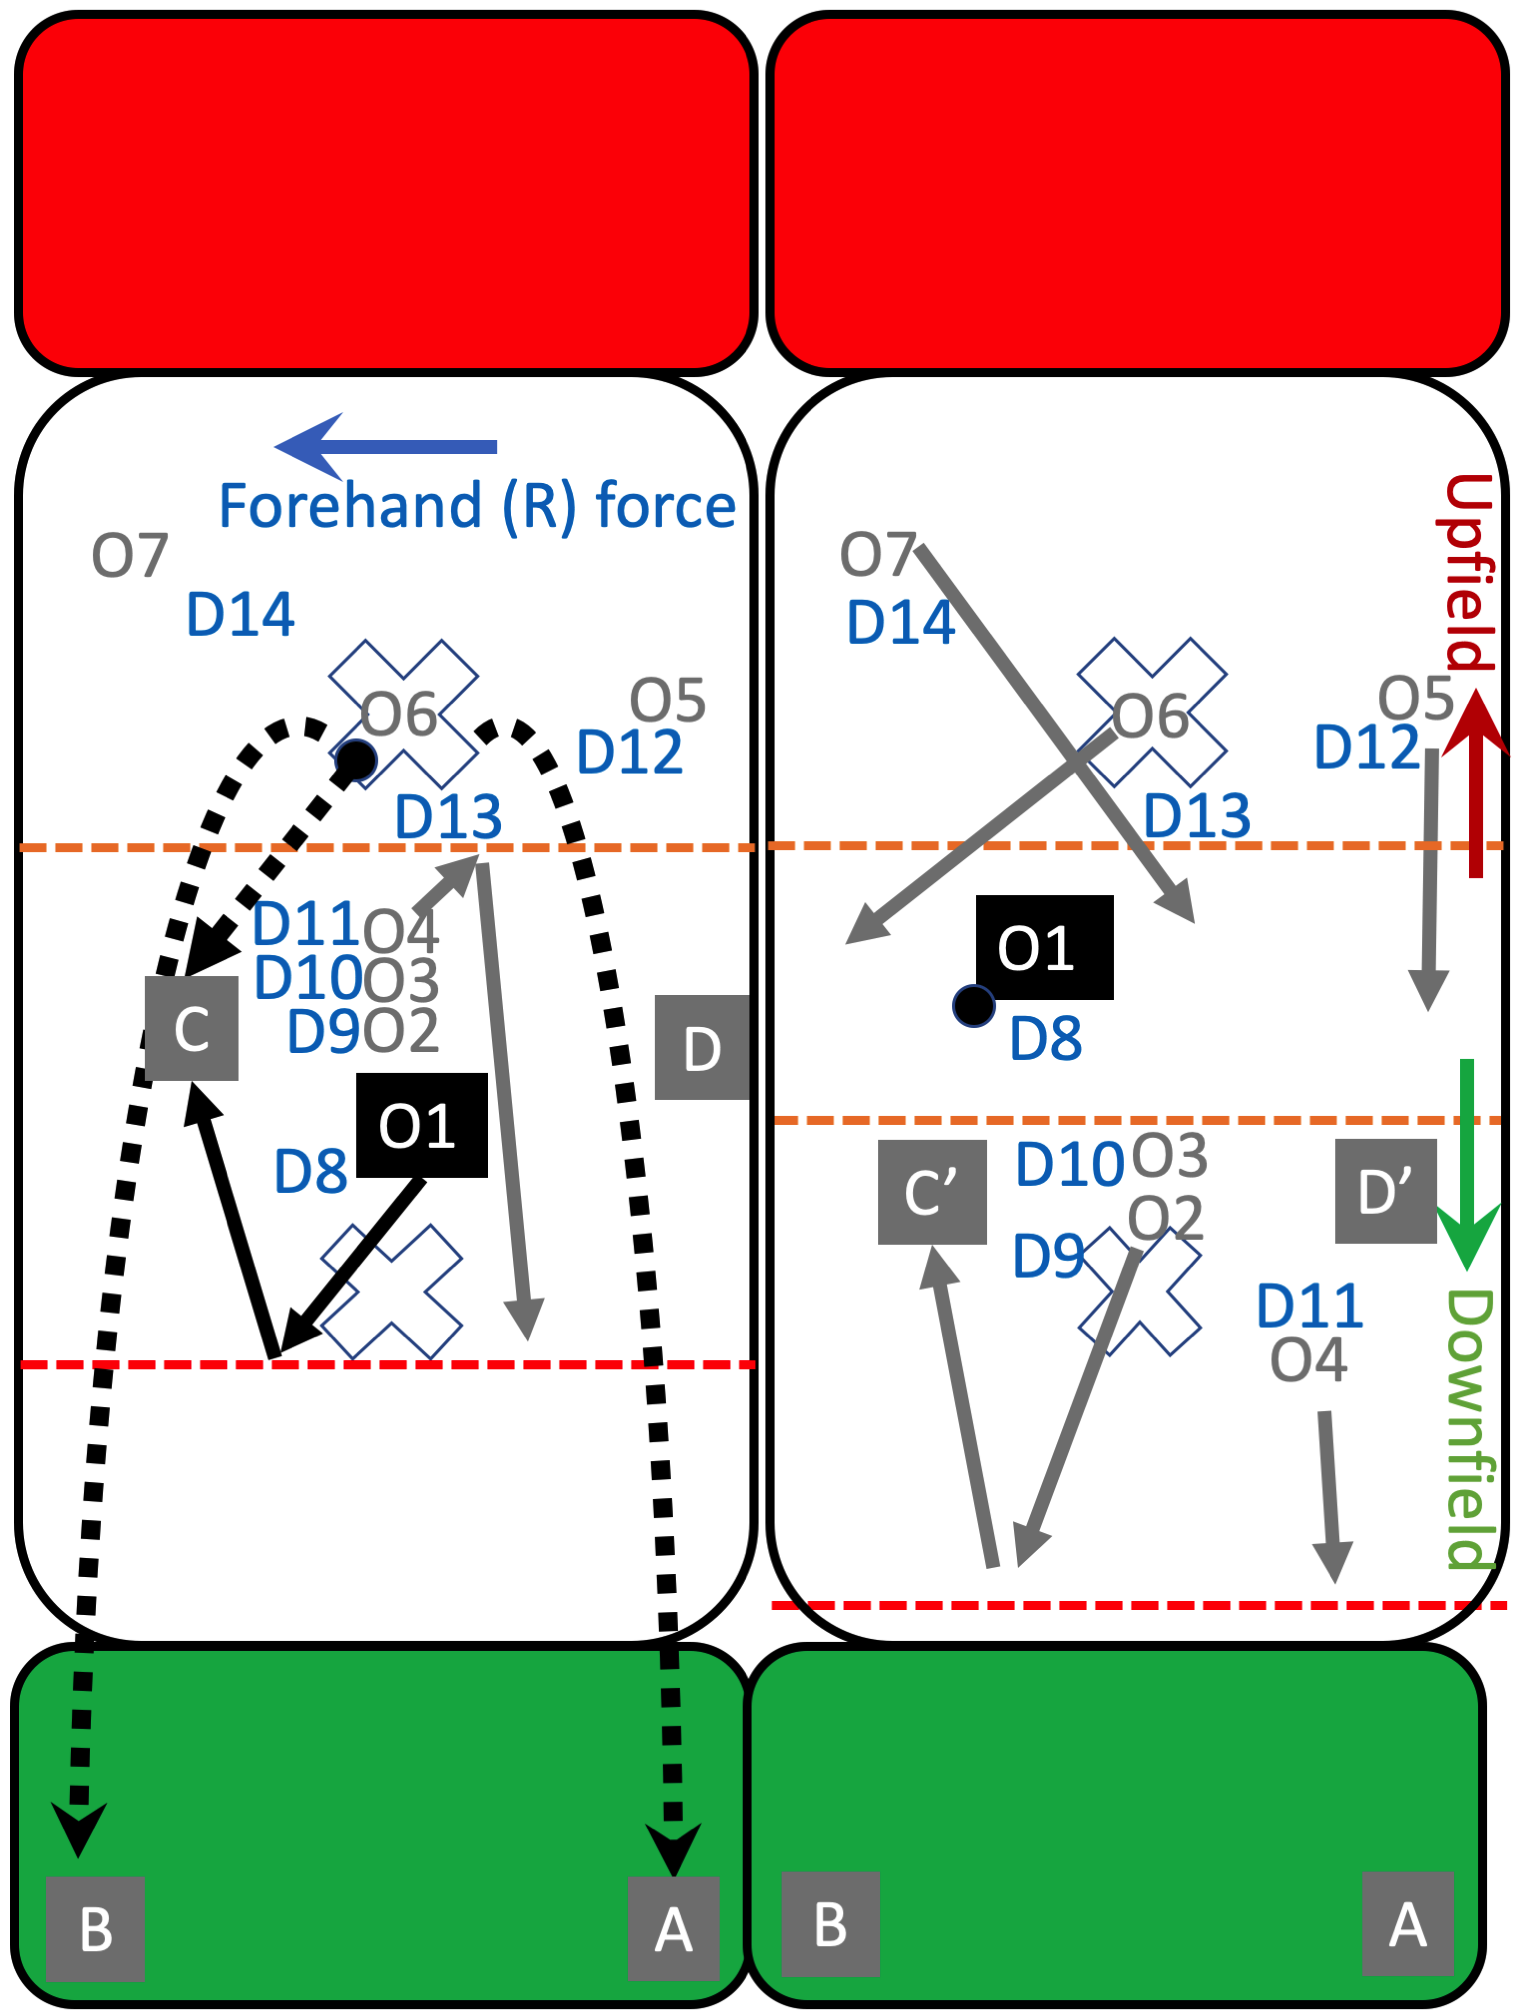
\includegraphics[width=\linewidth]{O1-vertical}
 % \caption{Vertical stack: 
%  starting position (left),
%  and development (right)}
%  \label{fig:O1-vertical}
% \end{marginfigure}


\end{document}
